\chapter{Demo}\label{ch:demo}

\section{Requisiti}\label{sec:demo-requisiti}

\subsection{Business}\label{subsec:demo-business}
L'obiettivo della demo è quello di permettere all'utente di avere una dimostrazione di applicazione del framework
ECScala.
Per farlo, si deve realizzare la simulazione del moto di palle da biliardo su un tavolo da gioco per la quale è
stato individuato il seguente requisito di business:
\begin{enumerate}[label=\textbf{\ref{subsec:demo-business}.\arabic*}]
    \item \label{itm:db1} Deve essere messa a disposizione un'interfaccia grafica che mostri e permetta d'interagire
    con la simulazione.
\end{enumerate}

\subsection{Utente}\label{subsec:demo-utente}
I requisiti utente sono di seguito riportati sotto forma di \textit{user stories}, secondo lo schema
``\textit{As a [persona], I [want to], [so that]}''.
\begin{table}[H]
    \begin{tabular}{p{0.18\linewidth}p{0.76\linewidth}}
        \toprule
        \textbf{User-story 1} &                                                                                      \\
        \textbf{Who}          & Come utilizzatore della demo                                                         \\
        \textbf{What}         & Vorrei avviare facilmente la simulazione senza dover inserire parametri              \\
        \textbf{Why}          & Per osservare il movimento delle palle da biliardo \\
        \bottomrule
    \end{tabular}\label{tab:user-story-1}
\end{table}
\begin{table}[H]
    \begin{tabular}{p{0.18\linewidth}p{0.76\linewidth}}
        \toprule
        \textbf{User-story 2} &                                                                               \\
        \textbf{Who}          & Come utilizzatore della demo                                                  \\
        \textbf{What}         & Vorrei poter aggiungere più palle da biliardo sul tavolo                      \\
        \textbf{Why}          & Per verificare l'interazione con quelle già presenti  \\
        \bottomrule
    \end{tabular}\label{tab:user-story-2}
\end{table}
\begin{table}[H]
    \begin{tabular}{p{0.18\linewidth}p{0.76\linewidth}}
        \toprule
        \textbf{User-story 3} &                                                           \\
        \textbf{Who}          & Come utilizzatore della demo                              \\
        \textbf{What}         & Vorrei poter cambiare la velocità delle palle da biliardo \\
        \textbf{Why}          & Per cambiarne la direzione e far muovere quelle ferme   \\
        \bottomrule
    \end{tabular}\label{tab:user-story-3}
\end{table}
\begin{table}[H]
    \begin{tabular}{p{0.18\linewidth}p{0.76\linewidth}}
        \toprule
        \textbf{User-story 4} &                                                                   \\
        \textbf{Who}          & Come utilizzatore della demo                                      \\
        \textbf{What}         & Vorrei poter modificare i coefficienti di frizione e restituzione \\
        \textbf{Why}          & Per osservare come cambia il movimento delle palle da biliardo    \\
        \bottomrule
    \end{tabular}\label{tab:user-story-4}
\end{table}
\begin{table}[H]
    \begin{tabular}{p{0.18\linewidth}p{0.76\linewidth}}
        \toprule
        \textbf{User-story 5} &                              \\
        \textbf{Who}          & Come utilizzatore della demo \\
        \textbf{What}         & Vorrei un tasto reset        \\
        \textbf{Why}          & Per riavviare la simulazione \\
        \bottomrule
    \end{tabular}\label{tab:user-story-5}
\end{table}

\subsection{Funzionali}\label{subsec:demo-funzionali}
Di seguito si elencano i requisiti funzionali individuati per il funzionamento della demo:
\begin{enumerate}[label=\textbf{\ref{subsec:demo-funzionali}.\arabic*}]
    \item \label{itm:df1} Gestire le collisioni tra le palle e i bordi dell'interfaccia grafica oltre che le collisioni
    tra le stesse.
    \item \label{itm:df2} Tenere conto della frizione nel calcolo della velocità
    \item \label{itm:df3} Renderizzare le palle da biliardo iniziali
    \item \label{itm:df4} Permettere cambio di velocità
    \item \label{itm:df5} Permettere l'aggiunta di palle
    \item \label{itm:df6} Permettere di spostare palle
\end{enumerate}


\section{Design architetturale}\label{sec:demo-design-architetturale}
A seguito dell'analisi dei requisiti definiti nella sezione precedente, si è realizzato il design architetturale di
massima riportato in Figura~\ref{fig:demo-architechture}.

Il pattern architetturale scelto è ECS, poiché si presta bene a questo genere di applicazioni.
Come mostrato in Figura~\ref{fig:demo-architechture}, si possono individuare alcuni sistemi fondamentali:
\begin{itemize}
    \item \textbf{RenderSystem:} per effettuare il rendering dei diversi elementi grafici
    \item \textbf{FrictionSystem:} per considerare l'apporto dell'attrito nel movimento delle palle
    \item \textbf{CollisionSystem:} per gestire le collisioni delle palle
    \item \textbf{BallCreationSystem:} per aggiungere nuove palle
    \item \textbf{BallEditingSystem:} per modificare velocità o posizione delle palle
    \item \textbf{BallSelectionSystem:} per selezionare delle palle
\end{itemize}

\begin{figure}[H]
    \centering
    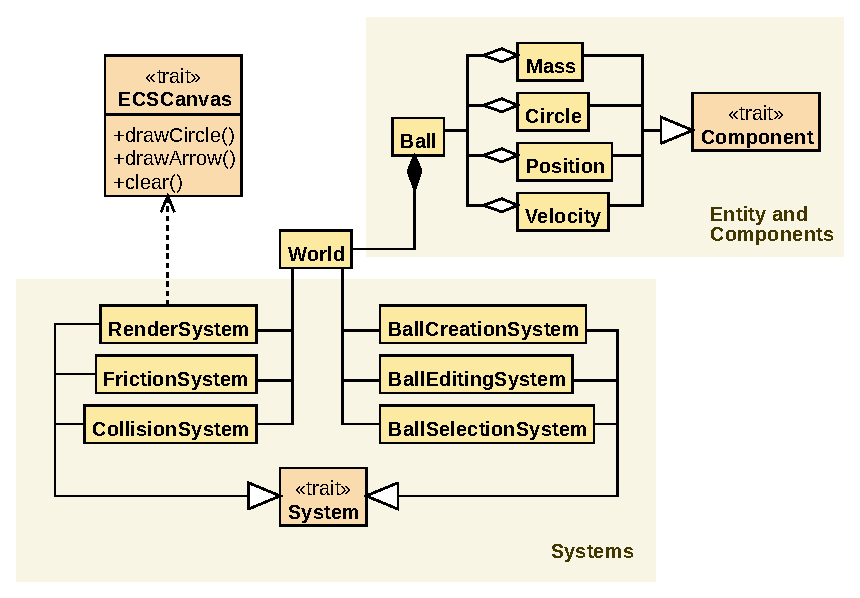
\includegraphics[width=\textwidth]{./img/DemoArchitecture}
    \caption{Design architetturale della demo.}
    \label{fig:demo-architechture}
\end{figure}

\section{Design di dettaglio}\label{sec:demo-design-di-dettaglio}
È stato ulteriormente approfondito il design architetturale dividendo i sistemi in sistemi più piccoli
dai compiti ben circoscritti.
Il design di dettaglio finale è riportato in Figura~\ref{fig:demo-detail},
tutti i sistemi individuati sono:
\begin{itemize}
    \item \textbf{AutoPauseSystem:} mette in automatico il gioco in pausa quando nessuna palla è più in movimento
    \item \textbf{BallCreationRenderingSystem:} si occupa di renderizzare la fase di creazione di una nuova palla
    \item \textbf{BallCreationSystem:} aggiunge una nuova palla al mondo
    \item \textbf{BallSelectionSystem:} seleziona una palla quando viene cliccata
    \item \textbf{ClearCanvasSystem:} pulisce il canvas a ogni frame
    \item \textbf{CollisionSystem:} calcola le nuove velocità di eventuali entità che collidono fra loro
    \item \textbf{FrictionSystem:} calcola le nuove velocità considerando il coefficente di frizione
    \item \textbf{MovementSystem:} calcola le nuove posizioni delle palle
    \item \textbf{RegionAssignmentSystem:} assegna le palle a specifiche regioni del canvas
    \item \textbf{RenderSystem:} effettua il rendering delle palle
    \item \textbf{VelocityArrowSystem:} disegna il vettore della velocità quando si modifica la velocità a una palla
    \item \textbf{VelocityEditingSystem:} assegna il nuovo valore di velocità a una palla
    \item \textbf{WallCollisionSystem:} gestisce le collisioni delle palle con i muri
\end{itemize}

\begin{figure}[H]
    \centering
    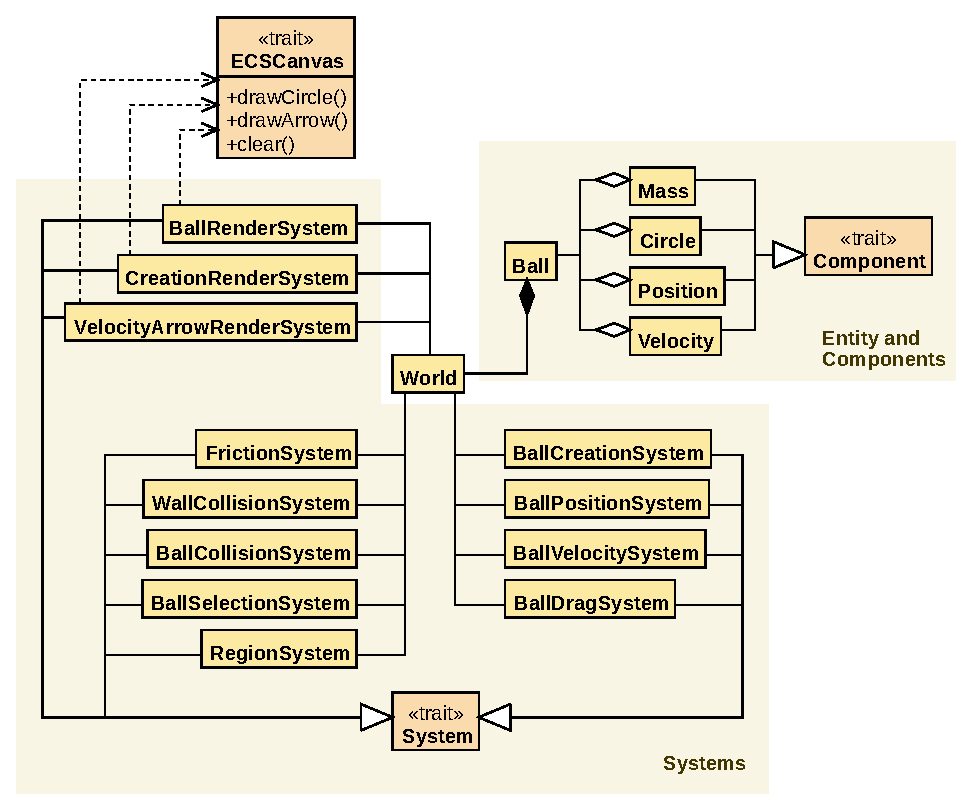
\includegraphics[width=\textwidth]{./img/Demo}
    \caption{Design di dettaglio della demo, i sistemi sono stati esplosi in sistemi più piccoli dai compiti ben circoscritti.}
    \label{fig:demo-detail}
\end{figure}

Inoltre, per ridurre la complessità nell'implementazione dei sistemi si è deciso di demandare la gestione della
posizione delle palle nello spazio bidimensionale allo \texttt{SpacePartitionContainer}.
Sono state realizzate due interfaccie che separano le operazioni di modifica da quelle di lettura dello stato;
in questo modo si può garantire che solo i sistemi che hanno bisogno di aggiungere elementi al container possano
effettivamente farlo.
Una trattazione più approfondita della logica di funzionamento del container si trova alla
Sottosezione~\ref{subsubsec:container}.

\subsection{Macchina a stati finiti}\label{subsec:macchina-a-stati-finiti}
Le macchine a stati finiti (FSM) consentono di descrivere formalmente il comportamento di un sistema.
Si è quindi scelto tale formalismo per descrivere il funzionamento della simulazione.

Sono stati identificati sei stati: \textit{Pause}, \textit{Play}, \textit{Add Balls}, \textit{Select Ball},
\textit{Change Velocity} e \textit{Dragging}.
A seguito della definizione degli stati del sistema, sono stati definiti i loro eventi di transizione.
Di seguito viene riportata la descrizione di tali eventi:
\begin{itemize}
    \item \texttt{PlayPauseBtn.clicked}: rappresenta la pressione del pulsante per eseguire o mettere in pausa la
    simulazione
    \item \texttt{AddBallBtn.clicked}: rappresenta la pressione del pulsante per l'aggiunta di palle alla simulazione
    \item \texttt{ChangeVelBtn.clicked}: rappresenta la pressione del pulsante per cambiare la velocità a una palla
    \item \texttt{Ball.selected}: rappresenta l'evento di selezione di una palla
    \item \texttt{Mouse.clicked}: rappresenta il singolo click del mouse
    \item \texttt{Mouse.dragging}: rappresenta l'evento di trascinamento del mouse
    \item \texttt{Mouse.released}: rappresenta l'evento di rilascio del tasto del mouse
\end{itemize}

In Figura~\ref{fig:fsm-demo} viene riportata la macchina a stati finiti utilizzata per descrivere il comportamento
della simulazione.

\begin{figure}[H]
    \centering
    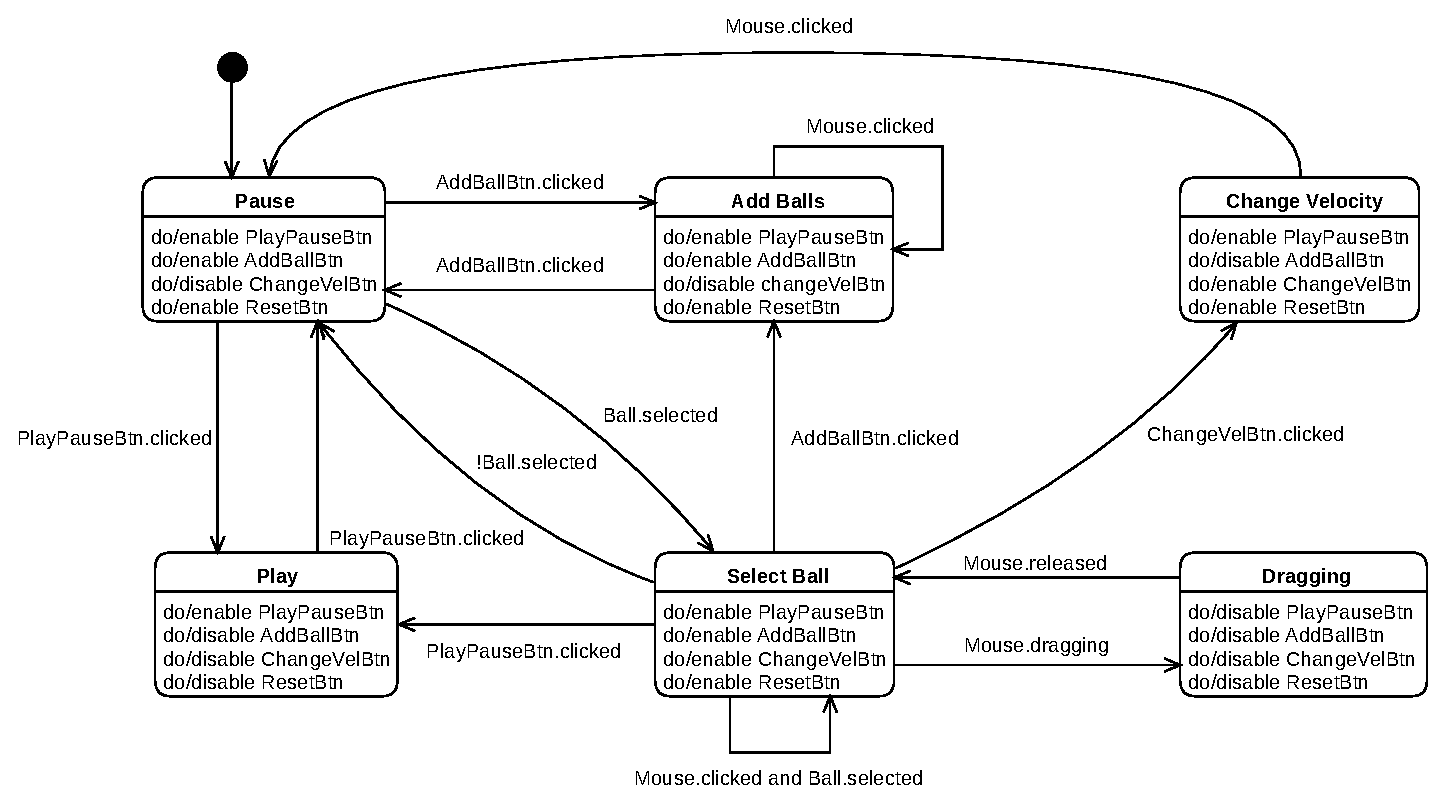
\includegraphics[width=\textwidth]{img/fsm-demo}
    \caption{Macchina a stati finiti che modella il flusso di esecuzione della demo.}\label{fig:fsm-demo}
\end{figure}

In una prima implementazione della demo si erano definiti oggetti globali che mantenessero lo stato della simulazione.
Ben presto ci si è resi conto della difficoltà nel gestire tutte le combinazioni dei campi dell'oggetto, oltre
ai vari bug che si verificavano durante l'implementazione della demo.
L'introduzione della macchina a stati ha portato diversi vantaggi: si è semplificata la gestione dello
stato della simulazione, le precondizioni di esecuzione dei sistemi fanno riferimento allo stato della FSM e non più
alla combinazione di più variabili booleane e la logica di aggiornamento dei componenti della GUI si è semplificata
notevolmente.
Grazie alla FSM è stato implementato un testing esaustivo delle precondizioni dei sistemi, esaminando tutte
le possibili configurazioni della FSM in unione agli eventi del mouse.
In questo modo è stato possibile individuare piccoli bug nell'implementazione dei sistemi.

\subsection{ECSCanvas}\label{subsec:ecscanvas}
Per non legarsi ad una specifica libreria grafica, si è deciso di introdurre una classe che esponesse metodi di alto livello
per disegnare le primitive necessarie (in particolare cerchio e linea) e ottenere le dimensioni dell'aria di disegno.
È stato inoltre deciso di introdurre il pattern Façade, descritto in Figura~\ref{fig:facade}, per nascondere la complessità della libreria ScalaFX e,
in particolare, della classe \texttt{Canvas}.

\begin{figure}[H]
    \centering
    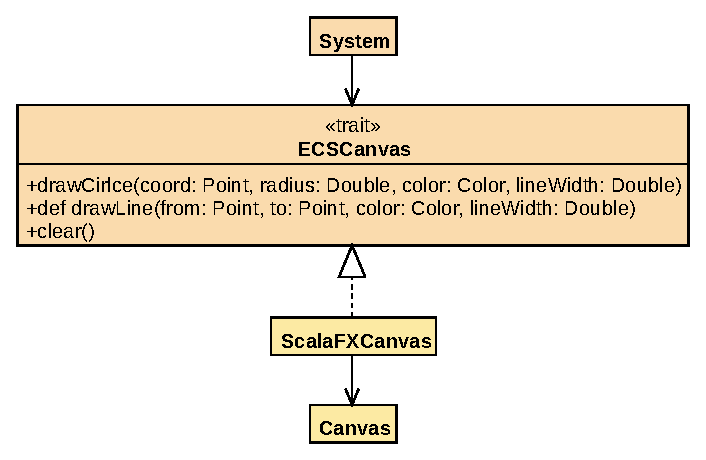
\includegraphics[width=\textwidth]{img/Facade}
    \caption{Utilizzo del pattern façade nella demo.}\label{fig:facade}
\end{figure}

\section{Implementazione}\label{sec:demo-implementazione}
Di seguito si riportano gli aspetti implementativi che meritano una trattazione più approfondita.

\subsection{Tecnologie utilizzate}\label{subsec:demo-tecnologie-utilizzate}
Anche per l'implementazione della demo ci sono stati problemi di incompatibilità con Scala 3:
in particolare è stata usata la libreria Mockito~\cite{mockito} invece di ScalaMock e non è stato possibile utilizzare
ScalaFXML che avrebbe fornito una sintassi idiomatica per usare JavaFX da Scala\@.
Per la realizzazione dell'interfaccia grafica è stata utilizzata la libreria ScalaFX~\cite{scalafx}\@.

\subsection{Cavalieri}\label{subsec:demo-cavalieri}
\subsubsection{Test dei sistemi}
Ogni sistema descritto nella Sezione~\ref{sec:demo-design-di-dettaglio} ha una specifica precondizione d'esecuzione
che determina, in base allo stato del gioco e allo stato del mouse, se il sistema può essere eseguito.
Testare tutte le possibili combinazioni di stato del gioco e stato del mouse avrebbe comportato la scrittura di codice
molto ripetitivo.
Perciò mi sono occupato di realizzare dei test che verificassero automaticamente che ogni sistema
fosse abilitato unicamente negli stati indicati e disabilitato in tutti i rimanenti.

La scrittura di un test delle precondizioni si limita quindi a indicare un costruttore del sistema in esame e
gli stati in cui questo dev'essere abilitato.
Un esempio di tale codice è riportato al Listato~\ref{lst:demo-prec-test}

\lstinputlisting[label={lst:demo-prec-test},
    caption=Esempio di test della correttezza delle precondizioni di un sistema.]
{code/demo-precondition-test.scala}

Il metodo \texttt{checkAllStates} utilizza un approccio di \textit{table-driven property testing} per effettuare
una scansione esaustiva di tutti i possibili stati e verificare che il sistema sia abilitato solo in quelli indicati.

\subsubsection{Test della GUI}
Un altro aspetto importante è stato verificare che la GUI realizzata rispettasse gli stati e le transizioni indicate
dalla FSM riportata in Figura~\ref{fig:fsm-demo};
per testare automaticamente la GUI è stata utilizzata la libreria TestFX~\cite{testfx}.

Dato uno stato della FSM vengono specificati alcuni elementi:
\begin{itemize}
    \item Le interazioni da svolgere con la GUI per raggiungere tale stato
    \item Quali bottoni devono essere abilitati o disabilitati nello stato
    \item Quali stati ulteriori possono essere raggiunti e, per ognuno di questi, quali interazioni devono essere svolte
    con la GUI per raggiungerlo
\end{itemize}
Date queste informazioni, un test risulta essere piuttosto semplice: viene raggiunto lo stato in esame, si verifica che
i bottoni siano nella configurazione richiesta e si controlla che tutti gli altri stati indicati siano effettivamente
raggiungibili svolgendo le operazioni indicate.

\subsection{Farabegoli}\label{subsec:demo-farabegoli}
\subsubsection{Game loop}
Il \textit{game loop} è il ciclo infinito che si occupa di eseguire tutti i sistemi dell'applicazione a ogni frame.

Mi sono occupato della sua realizzazione facendo uso della classe \texttt{AnimationTimer} già presente in ScalaFX\@.
Tale classe consente di eseguire del codice implementandolo nel metodo \texttt{handle}.
Questo metodo viene chiamato a ogni frame: un frame è renderizzato ogni $\approx16.6$ millisecondi per garantire 60 FPS
(Frames Per Second).
Il limite di 60 FPS è automaticamente garantito dalla classe, quindi non è necessario implementare una logica
di limitazione degli FPS\@.

La suddetta classe è stata concepita per essere utilizzata in un contesto OOP, per questa ragione è una classe astratta
che forza l'implementazione del metodo \texttt{handle}.
Ho quindi deciso di trasformare la classe affinché avesse un comportamento più funzionale.
A tal proposito ho creato un wrapper attorno alla classe per consentire di specificare l'handler del metodo direttamente
dal costruttore della classe mediante passaggio di funzione.

Nel Listato~\ref{lst:lstinputlisting3} è illustrato come è stato effettuato il wrapping della classe
\texttt{AnimationTimer}; per semplicità è stata omessa la parte di calcolo degli FPS\@.

\lstinputlisting[
    label={lst:lstinputlisting3},
    caption=Esempio d'implementazione del game loop mediante la classe \texttt{AnimationTimer}.
]{code/game-loop.scala}

Con l'\texttt{apply} è possibile specificare, mediante una lambda, il codice che deve essere eseguito a ogni
frame.
Con i metodi \texttt{start} e \texttt{stop} è possibile rispettivamente eseguire il game loop e fermarlo.

\subsubsection{FSM}
Mi sono occupato di realizzare la macchina a stati per gestire la logica del simulatore.
Per una trattazione dettagliata fare riferimento alla Sezione~\ref{subsec:macchina-a-stati-finiti}

\subsubsection{Interfaccia utente}
Mi sono occupato della realizzazione del'interfaccia grafica del simulatore;
a tal proposito si è fatto uso della libreria ScalaFX, la quale offre un DSL per la creazione d'interfaccie grafiche.

L'interfaccia si compone di una singola finestra che mostra una serie di bottoni per far interagire l'utente con la
simulazione, oltre a un pannello composto da due slider che consentono di configurare parametri di simulazione.
Al centro della finestra è presente un canvas che renderizza gli oggetti della simulazione.
L'interfaccia utente è stata sviluppata affinché risulti intuitiva e fornisca la massima semplicità d'uso all'utente.

\subsection{Di Domenico}\label{subsec:demo-di-domenico}

\subsubsection{Collision System}\label{subsubsec:container}
Il sistema principale che gestisce la simulazione è il \texttt{CollisionSystem}: questo implementa i calcoli necessari
per testare se c'è una collisione fra due corpi e, in caso affermativo, calcolarne le nuove velocità.

Sarebbe necessario controllare tutte le possibili coppie di corpi, ma questo presenta due importanti problemi:
\begin{itemize}
    \item ogni coppia di entità compare due volte anziché una
    \item la gran parte delle coppie di entità non porterà a una collisione, essendo troppo distanti fra loro
\end{itemize}

La soluzione a entrambi questi problemi è stata quella di applicare la tecnica di ottimizzazione detta
\textit{space partitioning}: si divide lo spazio (il piano in questo caso, essendo una simulazione 2D) in regioni
disgiunte affinché ogni entità appartenga a una e una sola di esse.

\subsubsection{SpacePartitionContainer}
Per ottimizzare i test di collisione è stato creato lo \texttt{SpacePartitionContainer}, che prende in ingresso
un'entità con tutti i componenti richiesti e la salva in una mappa che associa ogni regione (identificata da una coppia
di numeri interi) alla lista di entità che ne fanno parte.
Inoltre, lo \texttt{SpacePartitionContainer} dispone di un metodo per ottenere tutte le entità facenti parte di una
regione specificata e uno per iterare su tutte le regioni non vuote.

A questo punto, il \texttt{CollisionSystem} può diventare molto più efficiente: ora è sufficiente iterare su tutte le
regioni non vuote e testare le collisioni solo fra entità che fanno parte di un intorno bidimensionale di quelle
regioni, come mostrato in Figura~\ref{fig:space-partition}.
Per non processare due volte le coppie di entità, si costruiscono tutte le possibili combinazioni di lunghezza 2 e si
considera solo una metà dell'intorno, mentre l'altra verrà coperta nelle successive iterazioni delle regioni non vuote.

\begin{figure}[H]
    \centering
    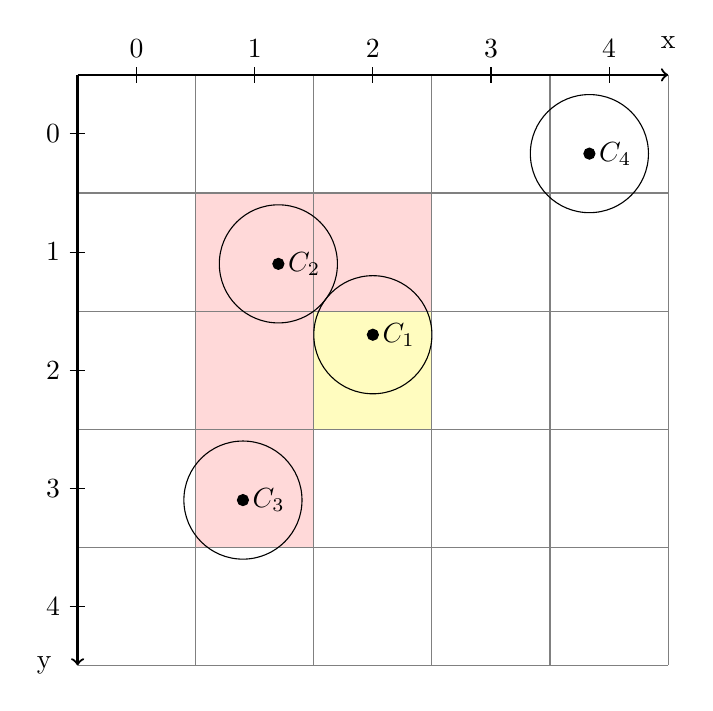
\begin{tikzpicture}
        \fill[red!15!white] (1.5, 6) rectangle (3, 1.5);
        \fill[red!15!white] (3, 6) rectangle (4.5, 4.5);
        \fill[yellow!25!white] (3, 4.5) rectangle (4.5, 3);
        \draw[step=1.5cm,gray,thin] (0, 0) grid (7.5, 7.5);
        \draw[thick,->] (0, 7.5) -- (7.5, 7.5) node[above=2mm] {x};
        \draw[thick,->] (0, 7.5) -- (0, 0) node[left=2mm] {y};
        \foreach \x [count=\i from 0] in {0, 1.5, 3, 4.5, 6}
        \draw (0.75+\x, 7.6) -- (0.75+\x, 7.4) node[above=2mm]{$\i$};
        \foreach \y [count=\i from 0] in {0, 1.5, 3, 4.5, 6}
        \draw (-0.1, 6.75-\y) -- (0.1, 6.75-\y) node[left=2mm]{$\i$};
        \draw (3.75, 4.2) circle (0.75cm);
        \filldraw[black] (3.75, 4.2) circle (2pt) node[anchor=west]{$C_1$};
        \draw (2.55, 5.1) circle (0.75cm);
        \filldraw[black] (2.55, 5.1) circle (2pt) node[anchor=west]{$C_2$};
        \draw (2.1, 2.1) circle (0.75cm);
        \filldraw[black] (2.1, 2.1) circle (2pt) node[anchor=west]{$C_3$};
        \draw (6.5, 6.5) circle (0.75cm);
        \filldraw[black] (6.5, 6.5) circle (2pt) node[anchor=west]{$C_4$};
    \end{tikzpicture}
    \caption{La regione in esame $(2, 2)$ controllerà solo se c'è collisione fra i cerchi con centro nelle regioni
    limitrofe (l'area rossa);
    si considera solo metà intorno per non contare due volte le coppie nelle iterazioni successive;
    si testerà quindi la collisione fra $C_1$ e $C_2$ e fra $C_1$ e $C_3$, mentre $C_4$ non viene preso in
    considerazione.}
    \label{fig:space-partition}
\end{figure}

\subsection{Vitali}\label{subsec:demo-vitali}
Nella parte di demo, oltre a \texttt{MovementSystem}, \texttt{FrictionSystem} e \texttt{RenderSystem},
mi sono occupata di una prima implementazione del \texttt{SimulationStatus}, che in seguito è stato adattato da
Farabegoli alla FSM sopra descritta.
Inoltre, ho implementato il trait \texttt{ECSCanvas}, descritto in Sezione~\ref{subsec:ecscanvas} che fornisce metodi per:
\begin{itemize}
    \item Disegnare un cerchio e una linea
    \item Ottenere le dimensioni dell'area di disegno
    \item Ripristinare l'area di disegno
\end{itemize}
Per il caso in esame, essendo stata scelta la libreria ScalaFX, ho realizzato anche la classe concreta
\texttt{ScalaFXCanvas} che estende il trait.
